\documentclass{article}
\usepackage{amsmath, amssymb, amsfonts, mathtools}
\usepackage[margin=1in]{geometry}
\usepackage{bbm}
\usepackage{graphicx}

\DeclareMathOperator{\EX}{\mathbb{E}\,}
\DeclareMathOperator{\IDF}{\mathbbm{1}}
\newcommand{\R}{\mathbb{R}}
\newcommand{\ind}{\perp \!\!\! \perp}

\title{Simulation Study}
\author{}
\date{}

\begin{document}
\maketitle

Both DGPs share the covariate and treatment-assignment mechanism:
\begin{align}
  X &\sim \mathrm{Uniform}(-1,1)^p, \quad p=5, \\
  e(x) &= \mathrm{sigmoid}(0.5\, x_1)
         = \frac{1}{1+\exp(-0.5\, x_1)}, \\
  W \mid X &\sim \mathrm{Bernoulli}\bigl(e(X)\bigr).
\end{align}
In both settings the censoring time is independent of the event time given covariates and treatment, and the administrative end of follow-up is $t_{\mathrm{end}}=5$.  The observed data are $Z = \min(D, C)$ and $\Delta = \IDF\{D \le C\}$.

%% ========================================================================
\section*{DGP~1: Heterogeneous Weibull}
%% ========================================================================

The event time in each arm follows a Weibull distribution whose scale depends on covariates:
\begin{align}
  D \mid X, W=w
    &\sim \mathrm{Weibull}\!\bigl(\alpha,\; \lambda_w(X)\bigr),
    &
  \alpha &= 1.5,
  \\
  \lambda_w(x)
    &= \exp\!\bigl(1 + 0.3\, x_1 + 0.5\, w\, x_2\bigr).
\end{align}
Here the Weibull parametrization is such that the survival function is
\[
  S_w(t \mid x)
  = \exp\!\Bigl(-\bigl(t / \lambda_w(x)\bigr)^{\alpha}\Bigr).
\]
The censoring time is exponential (i.e.\ Weibull with shape~$1$):
\[
  C \mid X \sim \mathrm{Weibull}(1,\, 5) \equiv \mathrm{Exp}(1/5).
\]
The true conditional average treatment effect is
\[
  \tau(t \mid x) = S_1(t \mid x) - S_0(t \mid x)
  = \exp\!\Bigl(-\bigl(t / \lambda_1(x)\bigr)^{1.5}\Bigr)
  - \exp\!\Bigl(-\bigl(t / \lambda_0(x)\bigr)^{1.5}\Bigr).
\]

Treatment-effect heterogeneity enters exclusively through~$x_2$: when $w=0$ the scale $\lambda_0(x)$ does not depend on~$x_2$, whereas $\lambda_1(x)$ does.  This makes the sign and magnitude of~$\tau(t\mid x)$ vary with~$x_2$.

%% ========================================================================
\section*{DGP~2: Weibull Mixture}
%% ========================================================================

Each arm's survival function is a three-component Weibull mixture:
\[
  S_w(t \mid x)
  = \sum_{k=1}^{3} \pi_k^{(w)}(x)\;
    \exp\!\Bigl(-\bigl(t / \lambda_k^{(w)}(x)\bigr)^{\alpha_k}\Bigr),
\]
with component shapes $(\alpha_1, \alpha_2, \alpha_3) = (1, 2, 3)$ and base log-scales $(\mu_1, \mu_2, \mu_3) = (0.8,\, 1.2,\, 1.8)$.

\paragraph{Control arm ($w=0$).}
The mixture weights are uniform and the scales depend only on~$x_1$:
\begin{align}
  \pi_k^{(0)}(x) &= \tfrac{1}{3}, \quad k=1,2,3, \\
  \lambda_k^{(0)}(x) &= \exp(\mu_k + 0.2\, x_1).
\end{align}

\paragraph{Treatment arm ($w=1$).}
Both the mixture weights and the scales depend on covariates:
\begin{align}
  \bigl(\pi_1^{(1)}(x),\; \pi_2^{(1)}(x),\; \pi_3^{(1)}(x)\bigr)
    &= \mathrm{softmax}\!\bigl(0.8\, x_2,\; 0,\; -0.8\, x_2\bigr), \\
  \lambda_k^{(1)}(x)
    &= \exp(\mu_k + 0.2\, x_1 + \gamma_k\, x_2),
    \quad (\gamma_1, \gamma_2, \gamma_3) = (0.5,\; 0,\; -0.3).
\end{align}

\paragraph{Censoring.}  Same as DGP~1:
\[
  C \mid X \sim \mathrm{Exp}(1/5).
\]

\paragraph{True CATE.}
\[
  \tau(t \mid x) = S_1(t \mid x) - S_0(t \mid x).
\]
This DGP produces richer heterogeneity than DGP~1: the treatment shifts both the mixture proportions and the component scales, so that the shape of the CATE curve --- not just its magnitude --- varies across subjects.

%% ========================================================================
\section*{Simulation Design}
%% ========================================================================

For each DGP, we evaluate six estimators of the time-varying CATE $\tau(t\mid x)$ across a range of training-set sizes $n \in \{500,\, 1000,\, 2000,\, 5000,\, 10000\}$.
For each sample size, $20$ independent datasets are drawn from the same distribution (using different random seeds), and all methods are fit on each dataset.

\paragraph{Methods compared.}
\begin{enumerate}
  \item \textbf{Cross-fitted AIR w/ MGD} --- the proposed method.  Nuisance functions (propensity, event/censoring survival in each arm) are estimated by $Q$-fold cross-fitting ($Q=3$); the CATE model is a covariate-gated mixture of $K=3$ Gamma survival differences (MGD).
  \item \textbf{Cross-fitted AIR w/ TP} --- same cross-fitted nuisances, but the CATE model is an unconstrained tensor-product of polynomial bases (degree~2 in covariates, $8$ time basis functions).
  \item \textbf{AIR w/ MGD (oracle nuis.)} --- the MGD CATE model trained with oracle (true) nuisance functions, isolating the CATE-modelling error.
  \item \textbf{AIR w/ TP (oracle nuis.)} --- the tensor-product CATE model with oracle nuisances.
  \item \textbf{Survival Forest T-learner} --- two separate random survival forests (200 trees each, minimum leaf size~10), one per treatment arm; $\hat\tau(t\mid x) = \hat S_1(t\mid x) - \hat S_0(t\mid x)$.
  \item \textbf{Survival Forest S-learner} --- a single random survival forest with treatment~$W$ as an additional covariate; predictions obtained by toggling $W=0/1$.
\end{enumerate}

\paragraph{Evaluation metric.}
Performance is measured by the integrated mean squared error (iMSE):
\[
  \mathrm{iMSE}
  = \frac{1}{n_{\mathrm{test}}} \sum_{i=1}^{n_{\mathrm{test}}}
    \sum_{m=0}^{M} \delta\,
    \bigl(\hat\tau(t_m \mid x_i) - \tau(t_m \mid x_i)\bigr)^2,
\]
where $(t_0, t_1, \dots, t_M)$ is a uniform grid of $M=50$ points on $[0, t_{\mathrm{end}}]$, $\delta = t_{\mathrm{end}} / M$ is the grid spacing, and the test set contains $n_{\mathrm{test}} = 1000$ subjects drawn independently from the same covariate distribution.

\paragraph{Training details.}
Nuisance models are trained for $80$ epochs; the CATE model is trained for $300$ epochs with learning rate $5 \times 10^{-4}$.  The MGD encoder uses hidden layers of sizes $(64, 32)$.

\paragraph{Reference line.}
The convergence plots include as a horizontal reference the iMSE of the population-average time-varying ATE, $\bar\tau(t) = n_{\mathrm{test}}^{-1} \sum_i \tau(t \mid x_i)$.  Any method whose iMSE falls below this line is capturing individual-level heterogeneity beyond what the marginal treatment effect provides.

%% ========================================================================
\section*{Results}
%% ========================================================================

Figure~\ref{fig:convergence} shows the mean iMSE ($\pm\, 1$ standard error) over 20 replications as a function of the training-set size, on a log--log scale.

\begin{figure}[ht]
  \centering
  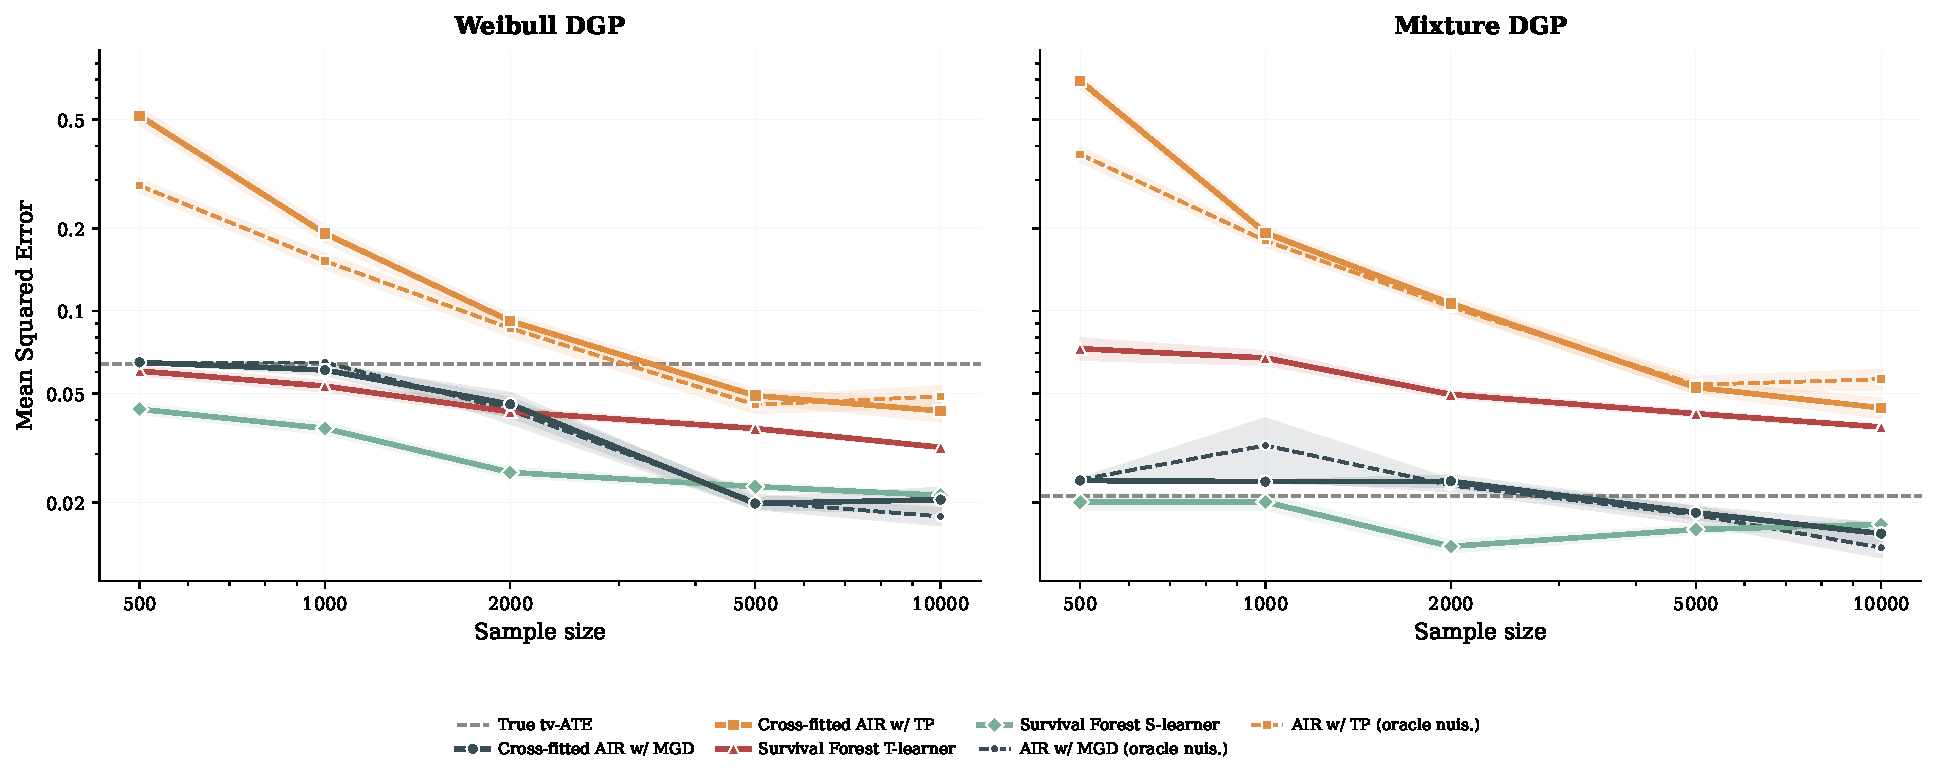
\includegraphics[width=\textwidth]{../examples/figures/simulation_convergence.pdf}
  \caption{Convergence of the integrated mean squared error (iMSE) as a function of the training-set size~$n$, for both DGPs.  Solid lines correspond to methods that estimate their own nuisance functions; dashed lines use oracle (true) nuisances.  The grey dashed horizontal line is the iMSE of the population-average time-varying ATE.  Shaded bands indicate $\pm\, 1$ standard error over $20$ replications.}
  \label{fig:convergence}
\end{figure}

Several findings emerge from the convergence plots.

\paragraph{Quasi-oracle property.}
Across both DGPs, the iMSE of Cross-fitted AIR w/ MGD (solid teal) decreases at essentially the same rate as its oracle counterpart AIR w/ MGD (dashed teal), which uses the true propensity, event-time, and censoring survival functions.
This demonstrates the quasi-oracle property of the cross-fitted AIR estimator: the additional error introduced by estimating the nuisance functions is asymptotically negligible relative to the CATE-modelling error.

\paragraph{Comparison with survival forest baselines.}
Cross-fitted AIR w/ MGD achieves lower iMSE than the Survival Forest T-learner across both DGPs and all sample sizes.
It also achieves lower iMSE than the Survival Forest S-learner in the Weibull DGP at large sample sizes ($n \ge 5000$), and is competitive with it in the Mixture DGP.
The S-learner benefits from pooling data across arms but does not directly target the treatment-effect contrast, which limits its ability to adapt to complex heterogeneity patterns as $n$ grows.

\paragraph{Benefit of structural constraints.}
The constrained Gamma mixture model (MGD) consistently outperforms the unconstrained tensor-product basis (TP), both in the cross-fitted and oracle settings.
The structural constraints of the MGD --- $\tau(0 \mid x) = 0$, $|\tau(t \mid x)| \le 1$, and $\tau(t \mid x) \to 0$ as $t \to \infty$ --- encode known properties of survival-function differences and reduce the effective model complexity, leading to faster convergence especially at smaller sample sizes.

\paragraph{Heterogeneity recovery.}
All methods eventually fall below the population-average tv-ATE reference line, confirming that they capture individual-level treatment-effect heterogeneity.  Cross-fitted AIR w/ MGD crosses this threshold at the smallest sample size among the cross-fitted methods.

%% ========================================================================
\section*{Illustrative Example: Structural Constraints in Practice}
%% ========================================================================

The time-varying CATE $\tau(t \mid x) = S_1(t \mid x) - S_0(t \mid x)$ is not an arbitrary function of time.  Because it is defined as a difference of two survival functions, it must satisfy several structural constraints:
\begin{enumerate}
  \item \textbf{Zero at time zero.}  $\tau(0 \mid x) = 0$, because $S_1(0 \mid x) = S_0(0 \mid x) = 1$ --- everyone is alive at the moment they receive treatment.
  \item \textbf{Vanishes at infinity.}  $\tau(t \mid x) \to 0$ as $t \to \infty$, because $S_1(t \mid x) \to 0$ and $S_0(t \mid x) \to 0$ --- eventually everyone dies regardless of treatment.
  \item \textbf{Bounded between $-1$ and $+1$.}  $|\tau(t \mid x)| \le 1$, because both $S_0$ and $S_1$ take values in $[0,1]$.
  \item \textbf{Continuity.}  $\tau(\cdot \mid x)$ is continuous, because survival functions of absolutely continuous event-time distributions are continuous.
\end{enumerate}

Figure~\ref{fig:cate_curves} illustrates these constraints on a single test observation from the Weibull DGP.  The true tv-CATE (grey dashed) satisfies all four properties by construction.

\begin{figure}[ht]
  \centering
  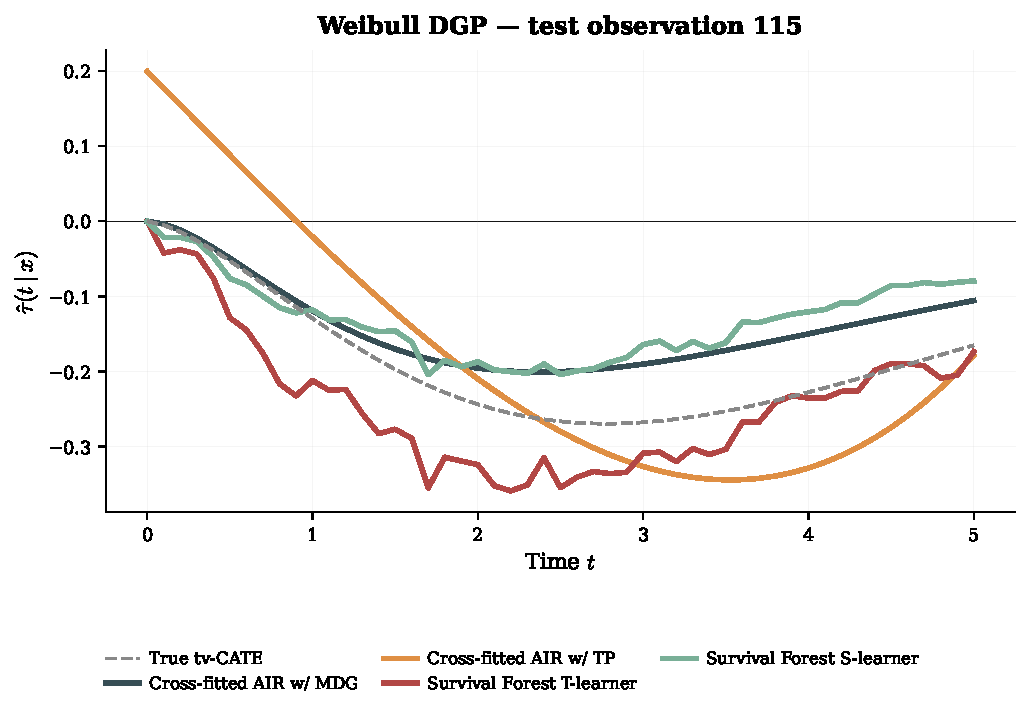
\includegraphics[width=0.85\textwidth]{../examples/figures/cate_curves.pdf}
  \caption{Predicted time-varying CATE $\hat\tau(t \mid x)$ for a single test observation (Weibull DGP, $n = 2000$ training samples).  The true tv-CATE is shown as a grey dashed curve.  Only non-oracle methods are displayed.}
  \label{fig:cate_curves}
\end{figure}

The MGD parametrization used by Cross-fitted AIR w/ MGD enforces all four constraints by construction, and its predicted curve closely tracks the true tv-CATE.
In contrast, the other methods violate one or more of these properties, as visible in Figure~\ref{fig:cate_curves}:

\begin{itemize}
  \item The \textbf{Survival Forest} methods (both T-learner and S-learner) produce step-function estimates that are \emph{not continuous}, because random survival forests aggregate Kaplan--Meier--type step functions across trees.
  \item The \textbf{tensor-product} parametrization does not enforce $\tau(0 \mid x) = 0$: on the figure, its predicted curve is visibly non-zero at $t = 0$.  Without this anchor point, the model must spend capacity learning a constraint that the MGD satisfies for free.
\end{itemize}

These constraint violations are not merely aesthetic.  A model that must learn structural properties from data rather than encoding them a priori has higher effective complexity, which translates into slower convergence of the iMSE --- precisely what the convergence plots in Figure~\ref{fig:convergence} confirm.  The MGD's built-in constraints reduce the hypothesis space to functions that are \emph{a priori} consistent with survival-function differences, yielding more efficient estimation.

\end{document}
